\section{Arbeid}
\subsection{Wat is arbeid?}
Arbeid is een vorm van energieoverdracht die plaatsvindt wanneer een kracht wordt uitgeoefend op een object en het object zich verplaatst in de richting van die kracht.
In de context van thermische fysica, wordt arbeid vaak geassocieerd met processen waarbij een systeem energie verliest of wint door middel van mechanische interacties.

\begin{definition}
    \textbf{Uitwendige Arbeid}: Arbeid die wordt verricht door een systeem op zijn omgeving, of door de omgeving op het systeem, als gevolg van mechanische interacties.
\end{definition}
\medskip
\begin{definition}
    \textbf{Inwendige Arbeid}: Arbeid die wordt verricht binnen een systeem, als gevolg van interne krachten en processen. \footnote{Een warme bal maakt nog steeds dezelfde beweging als een koude bal, maar er is wel een verschil in de interne energie, dus een verschil in inwendige arbeid.}
\end{definition}
\medskip
\begin{definition}
    \textbf{Positieve Arbeid}: Arbeid verricht op een systeem door zijn omgeving. \(\vec{e}_r = \vec{e}_F\)
\end{definition}
\medskip
\begin{definition}
    \textbf{Negatieve Arbeid}: Arbeid verricht door een systeem op zijn omgeving. \(\vec{e}_r = -\vec{e}_F\)
\end{definition}

\subsection{Arbeid bij volumeverandering}

\begin{figure}[ht]
    \centering
    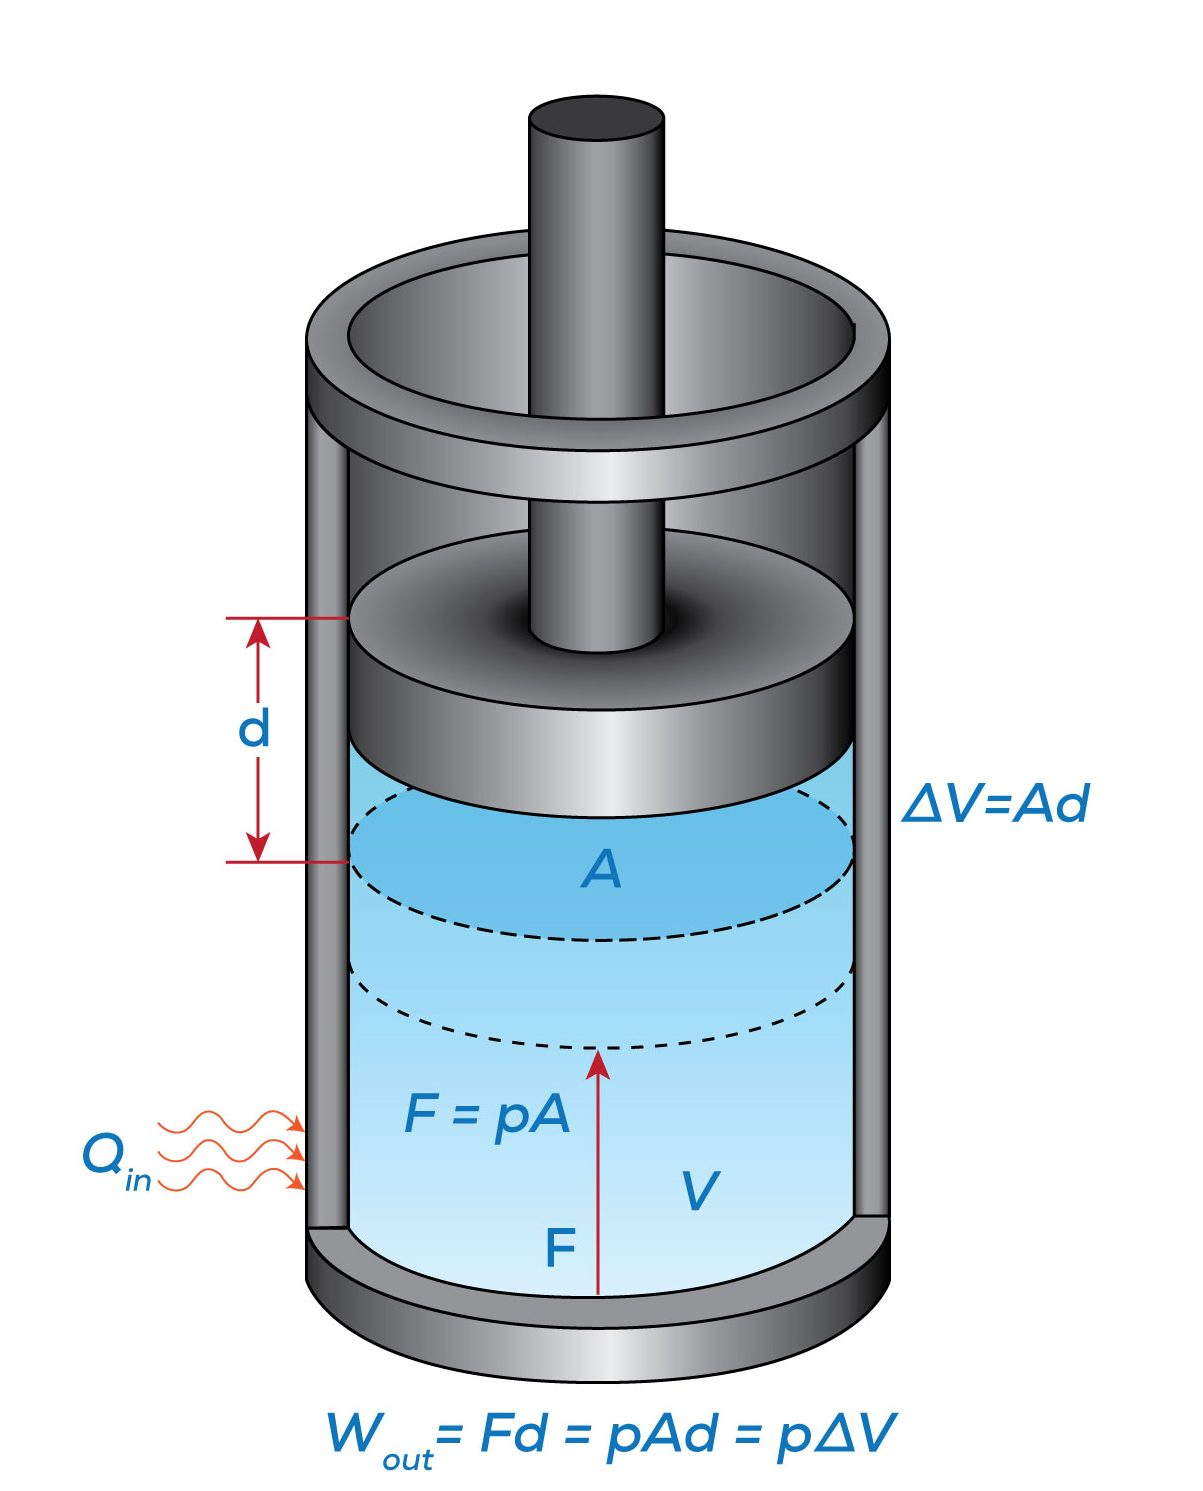
\includegraphics[width=0.3\textwidth]{Foto's-Figuren/Fig.-4-4_boundary-work1-e1626459353689.jpg}
    \caption{Arbeid verricht door een gas tijdens compressie. De kracht \(F\) werkt op de zuiger, waardoor deze zich verplaatst met een afstand \(dx\). De arbeid \(dW\) wordt gegeven door \(dW = F \cdot dx\). \footnotesize \copyright{Kh1604 is licensed under a CC BY-SA (Attribution ShareAlike) license}}
    \label{fig:work-gas-compression}
\end{figure}

\[
dW = F \cdot dx = -PAdx = -PdV
\]

Een negatief teken betekent dat een volumevergroting gepaard gaat met een negatieve arbeid, terwijl een volumeverkleining gepaard gaat met een positieve arbeid. 

Voor een quasistatisch proces geldt:
\begin{equation}
    \label{eq:hydrostatische-arbeid-algemeen}
    W = - \int_{V_i}^{V_f} PdV
\end{equation}

\begin{figure}[ht]
    \centering
    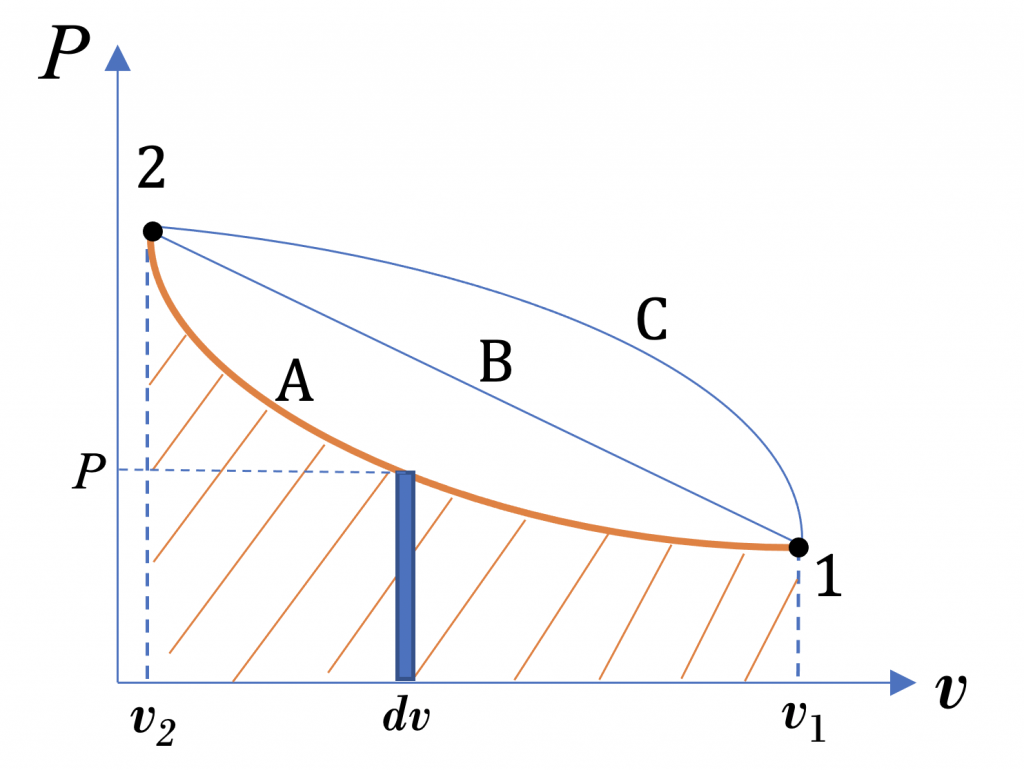
\includegraphics[width=0.3\textwidth]{Foto's-Figuren/P-v-for-boundary-work-1024x770.png}
    \caption{PV-diagram van een gas. De arbeid verricht door het gas tijdens een proces wordt gegeven door de oppervlakte onder de curve in het PV-diagram. \footnotesize \copyright{ Kh1604 is licensed under a CC BY-SA (Attribution ShareAlike) license}}
    \label{fig:work-gas-pv}
\end{figure}

Voor een quasistatisch proces is de arbeid gelijk aan de oppervlakte onder de curve in het PV-diagram. Stel we gaan van punt i naar punt f met een volume compressie:
\[
W_{if} = - \int_{V_i}^{V_f} PdV
\]
Als we van dat punt terug gaan van punt f naar punt i (en dus eeen volume expansie hebben), dan is de arbeid:
\[
W_{fi} = - \int_{V_f}^{V_i} PdV
\]
Dit betekend dat we een cyclus kunnen maken waarbij geldt \(W_{if} = -W_{fi}\). Dit is voor een quasistatisch proces langs heetzelfde pad!

Onze conventie voor cyclussen is als volgt: wijzerzin betekend dat er negatieve arbeid wordt verricht, terwijl tegenwijzerzin betekend dat er positieve arbeid wordt verricht op het systeem. Typisch zijn koelmachines tegenwijzerzin, terwijl warmtemachines wijzerzin zijn.

\subsection{Padafhankelijke Arbeid}

\begin{derivation}
    \textbf{Arbeid is padafhankelijk}: Stel we kunnen van punt 1 naar punt 2 gaan via twee verschillende paden, namelijk pad A en pad C. (Zie figuur \ref{fig:work-gas-pv}.)
    We kunnen ook een cyclus maken door van punt 1 naar punt 2 te gaan via pad C, en vervolgens terug te gaan van punt 2 naar punt 1 via pad A. De netto arbeid verricht tijdens deze cyclus is:
    \begin{align*}
        W_{cyclus} &= W_{21}(C) + W_{12}(A) 
        = -|W_{21}(C)| + |W_{12}(A)| < 0 
        \implies |W_{21}(C)| > |W_{12}(A)| \\
    \end{align*}
    Als we nu proces A van 2 naar 1 laten verlopen, dan is de netto arbeid:
    \begin{align*}
        W_{21}(A) &= -W_{12}(A) <0 \implies |W_{21}(A)| = |W_{12}(A)| \\ 
    \end{align*}
    Uit \(|W_{21}(C)| > |W_{12}(A)|\) en \(|W_{21}(A)| = |W_{12}(A)|\) volgt dat \(|W_{21}(C)| > |W_{21}(A)|\). (Of stel dat beide negatief zijn, dan is \(W_{21}(C) < W_{21}(A)\).)
    Dit betekent dat de arbeid die wordt verricht tijdens het proces van 2 naar 1 via pad C groter is dan de arbeid die wordt verricht tijdens het proces van 2 naar 1 via pad A.
    \qed
\end{derivation}
\medskip
\begin{postulate}
    \textbf{Arbeid is padafhankelijk!}
\end{postulate}

Stel we hebben een  \textbf{isobaar} proces, dan wordt de arbeid:
\begin{equation}
\label{eq:isobare-arbeid}
W = -P \int_{V_i}^{V_f} dV = -P(V_f - V_i) \qquad (P = cst)
\end{equation}
Voor een  \textbf{isochoor} proces is de arbeid triviaal 0.

\textbf{Isotherme arbeid} is dan weer een ander verhaal:
\[
W = - \int_{V_i}^{V_f} P(V)dV
\]
Waarbij de toestandsfunctie \(P(V, T)\) nu enkel van het volume afhangt \(P(V)\). 
Voor een ideaal gas is \(P = \frac{nRT}{V}\), dus de arbeid wordt:
\begin{equation}
\label{eq: isotherme-arbeid-ideaal-gas}
W = - \int_{V_i}^{V_f} \frac{nRT}{V}dV = -nRT \ln\left( \frac{V_f}{V_i} \right) \qquad (T = cst)
\end{equation} 

\textbf{Isotherme toename van druk op een vaste stof}:
\[
dV = \left( \frac{\partial V}{\partial P} \right)_T dP = - \kappa V dP \qquad (T = cst)
\]
Waar we formule \eqref{eq:isothermische-drukbaarheid} hebben gebruikt, nu volgt dat de arbeid:
\begin{equation}
\label{eq: isotherme-arbeid-vast-stof}
W = - \int_{P_i}^{P_f} \kappa VP  dP \qquad (T = cst)
\end{equation} 

Het is niet moeilijk te realiseren dat als de temperatuur constant is, een vaste stof niet veel zal uitzetten, waardoor we \(V,\kappa \approx cst\) kunnen beschouwen.

\[
W \approx \frac{\kappa V}{2} (P_f^2 - P_i^2) = \frac{\kappa m}{2\rho} (P_f^2 - P_i^2) \qquad (T = cst)
\]
Waar we gebruik hebben gemaakt van \(V = \frac{m}{\rho}\) met \(m\) de massa en \(\rho\) de dichtheid van de vaste stof.

\subsubsection{De gespannen snaar herzien}

\(\dbar W = FdL  \implies W = \int_{L_i}^{L_f} F dL\)

Herinner de wet van hooke, \(F = k(L - L_0)\), waarbij \(k\) de veerconstante is en \(L_0\) de natuurlijke lengte van de veer. De arbeid wordt:
\[W = \int_{L_i}^{L_f} k(L - L_0) dL = \frac{k}{2} \left( (L_f - L_0)^2 - (L_i - L_0)^2 \right)\]

\subsubsection{Oppervlaktefilm herzien}

\( \dbar W = Fdx = 2 \gamma ldx \). De oppervlakte van de film is \(A = 2lx\) (langs 2 kanten), dus \(dA = 2ldx\). De arbeid wordt:

\[\dbar W = \gamma dA \implies W = \int_{A_i}^{A_f} \gamma dA\]

\subsubsection{Elektrolyse cel herzien}

\( \dbar W = V_\epsilon dQ \) met \(dQ\) het aantal verplaatste elektronen inde cel tijdens de reactie en \(V_\epsilon\) de elektrische potentiaal. De arbeid wordt: 
\[W = \int_{Q_i}^{Q_f} V_\epsilon dQ = \int_{t_i}^{t_f} V_\epsilon \frac{dQ}{dt} dt = \int_{t_i}^{t_f} V_\epsilon I dt\]

\subsubsection{Verandering vd polarisatie van een diëlektricum herzien}

\begin{figure}[ht]
    \centering
    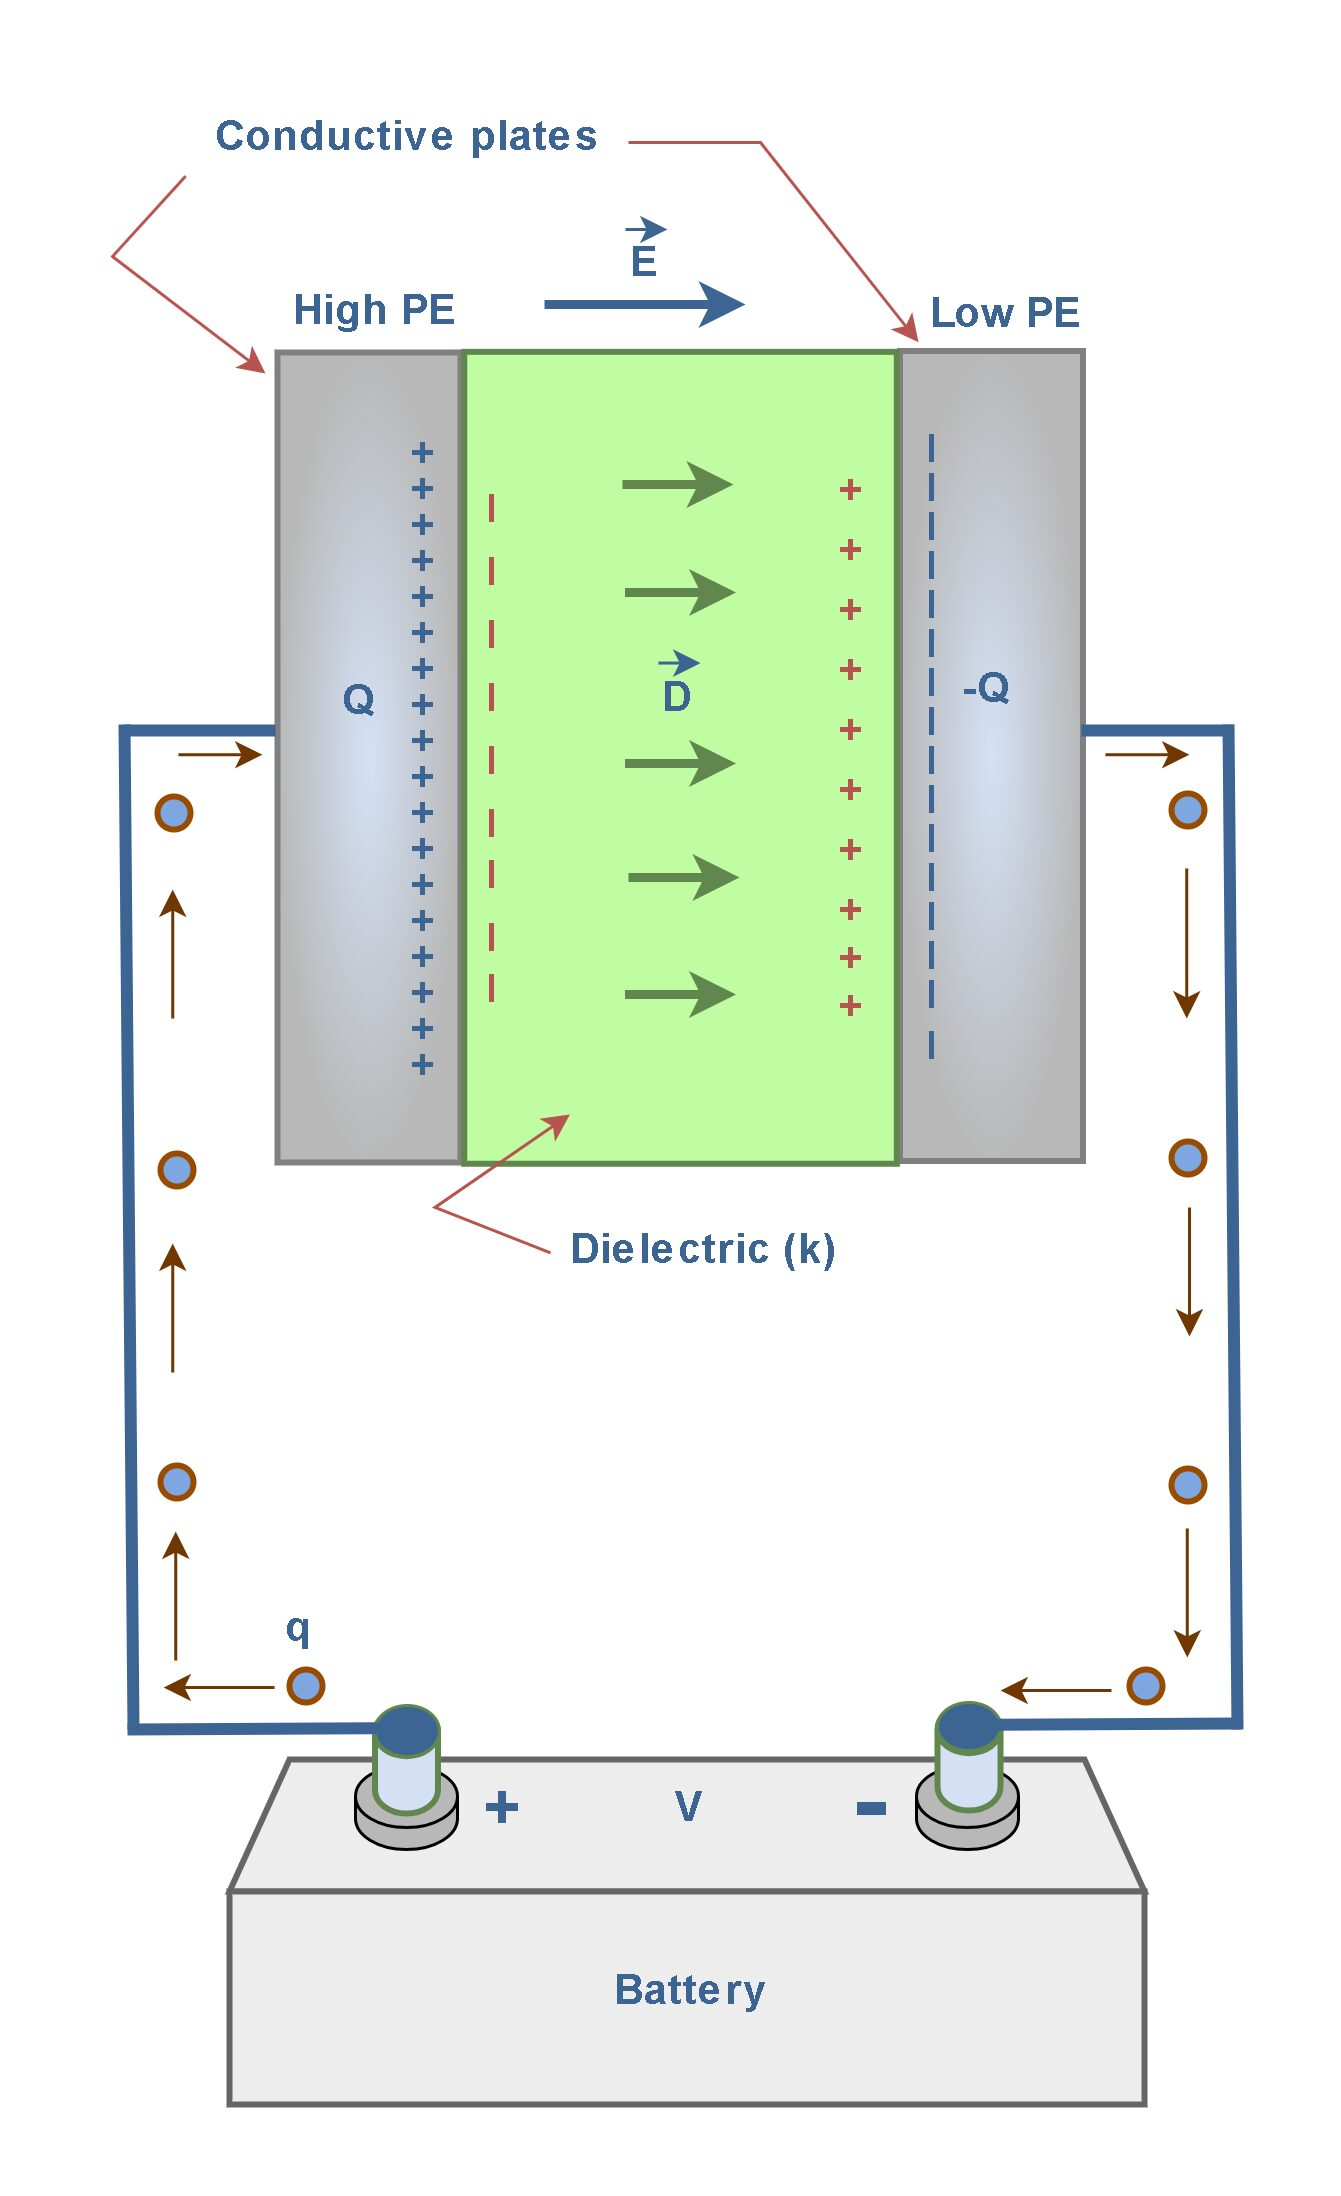
\includegraphics[width=0.5\textwidth]{Foto's-Figuren/Electric-Displacement.jpeg}
    \caption{Een diëlektricum tussen twee platen van een condensator. Wanneer er een elektrisch veld wordt aangelegd, worden de moleculen in het diëlektricum gepolariseerd, wat resulteert in een verandering van de polarisatie \(\Pi\) van het diëlektricum.
        \footnotesize \copyright{ September 29, 2024 by Kamran Jalilinia site: \url{https://www.electronics-lab.com/article/electric-displacement-and-electrostatic-energy/}}}
    \label{fig:di-electric-polarization}
\end{figure}


\(\dbar W = V_\epsilon dQ =EldQ\) met \(E = \frac{V_\epsilon}{l}\) het elektrische veld. (zie figuur \ref{fig:di-electric-polarization}) 

\(Q = A(\bm D \cdot \bm n) \) met \(\bm n\) de normaal op het oppervlak (in ons geval staat alles loodrecht dus wordt dit geen probleem).

\(\dbar W = ElAdD = EVdD \) met \(V\) nu het volume vh dielektricum (wordt constant beschouwd).

Uit \(\bm D = \epsilon_0 \bm E + \frac{\bm \Pi}{V} \implies dD = \epsilon_0 dE + \frac{d\Pi}{V}\) (\(V\) = cst) volgt:

\[\dbar W = EVdD = \epsilon_0 E dE V + E d\Pi\]

Doordat enkel de tweeede term de polarisatie beïnvloed negeren we de eerste term, en krijgen we:
\[\dbar W = E d\Pi \implies W = \int_{\Pi_i}^{\Pi_f} E d\Pi\]



\subsubsection{Verandering vd magnetisatie van een magnetisch materiaal herzien}

\begin{figure}[ht]
    \centering
    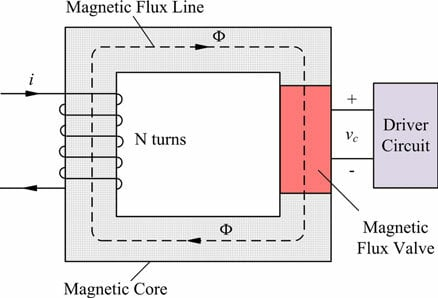
\includegraphics[width=0.5\textwidth]{Foto's-Figuren/arbeid-magnetisatie.jpeg}
    \caption{Een spoel met N windingen (magneetventiel). \footnotesize \copyright{ Magnetic Flux Valve: A Magnetoelectric Materials-Based Device for Conversion and Control of Electric Power - Scientific Figure on ResearchGate. Available from: \url{https://www.researchgate.net/figure/Simple-magnetic-circuit-containing-an-MFV_fig1_305802042} [accessed 10 May 2026] }}
    \label{fig:magnetization-work}
\end{figure}

Uit de inductiewet van Faraday volgt dat \( V_\epsilon = \frac{d\Phi}{dt} = -NA \frac{dB}{dt} \) met (\(A = cst\) en \(N\) het aantal windingen van de spoel zie figuur \ref{fig:magnetization-work}). 

\[\dbar W = -V_\epsilon dQ = -NA \frac{dB}{dt} dQ = -NA \frac{dQ}{dt} dB = -NAI dB \]

De magnetische veldsterkte \(H\) is gedefinieerd als \(H = \frac{NI}{l}\), dus \(NI = Hl \implies NIA = HV\).

\[\implies \dbar W = -HV dB\]

We moeten nog rekening houden met de differentiaal van \(B\). Herinner \(B = \mu_0(H + \frac{M}{V})\), dus \(dB = \mu_0(dH + \frac{dM}{V})\).

Dus \[\dbar W = -HV \mu_0(dH + \frac{dM}{V}) = -HV \mu_0 dH - H\mu_0 dM\]
We kunnen de eerste term negeren, omdat deze niet bijdraagt aan de verandering van de magnetisatie:

\[\dbar W = -\mu_0 H dM \implies W = -\mu_0 \int_{M_i}^{M_f} H dM\]

\subsection{Samengestelde Systemen}

Nu rest ons alleen nog te zien hoe we de arbeid kunnen berekenen voor samengestelde systemen, waarbij meerdere processen tegelijkertijd plaatsvinden.
In dit geval kunnen we de totale arbeid berekenen door de arbeid van elk proces afzonderlijk te berekenen en deze vervolgens op te tellen.
Dit is mogelijk omdat arbeid een additieve grootheid is, wat betekent dat de totale arbeid gelijk is aan de som van de arbeid van elk proces.

\begin{figure}[ht]
    \centering
    \includegraphics[width=0.5\textwidth]{Foto's-Figuren/Carnot_heat_engine_2.pdf}
    \caption{Een samengesteld systeem.  \footnotesize \copyright{Wikipedia contributor}}
    \label{fig:composite-system}
\end{figure}

Zo een samengesteld systeem kan vanalles zijn. Als we eens kijken naar 2 hydrostatische systemen A en B geïsolleerd met elkaar. Maar ze staan onrechtsreeks in contact met elkaar via een diathermischee wand met een reservoir C, dan hebben we 5 coordinaten: \(P_A, V_A, P_B, V_B\) en \(T_C =T\).

Er zijn 2 toestandsfuncties \( f_A(P_A,V_A, T) = 0\) en \(f_B(P_B,V_B, T) = 0\). De arbeid kan berekend worden aan de hand van:

\[\dbar W = -P_AdV_A - P_BdV_B\]

Dit kunnen we ook doen voor gelijk welke combinties van de voorgaande processen, zolang we maar de juiste toestandsfuncties en de bijbehorende differentiaalvergelijkingen hebben.

Algemeen geldt:
\[\dbar W = \sum_i Y_i dX_i\]
waarbij \(Y_i\) de veralgemeende kracht is die werkt op de veralgemeende verplaatsing \(X_i\). In het geval van ons eerdere hydrostatisch systeem is \(Y_i = -P\) en \(X_i = V\), terwijl in het geval van een gespannen snaar \(Y_i = F\) en \(X_i = L\) is, enzovoort.